\RequirePackage{lineno}
\documentclass[a4paper]{jpconf}
\usepackage{graphicx}
\usepackage{float}
\begin{document}

\linenumbers

\title{Glint: VM image distribution in an OpenStack multi-cloud environment}

\author{A.~Charbonneau, M.~Conklin, R.~Demarais, C.~Driemel, I.~Gable, C.~Leavett-Brown, 
M.~Paterson, R.J~Sobie, R.~Taylor}

\address{University of Victoria, Victoria, Canada}

\ead{rsobie@uvic.ca}

\begin{abstract}
The use of cloud computing is becoming widespread in the HEP community.  
In many instances, individual clouds are being federated to appear as a single
infrastructure that can be connected, for example, to the WLCG.
For a small number of clouds, it is relatively easy to manage the virtual
machine images on all the sites.  
However, as the number of clouds increases, then keeping track of the images
requires a more robust management system.
Glint is designed to manage virtual machine images on OpenStack clouds.
Glint makes it easy to distribute images on multiple clouds in a reliable and
error free manner. 
\end{abstract}

\section{Introduction}

The use of clouds in HEP is becoming a significant source of computing resources 
for MC production and data analysis.
There are a number of compelling reasons for the migration to clouds:
clouds give researchers quick and dynamic access to unused or opportunistic
resources;  sites find it easier to manage multiple project that have their
own specific software requirements; and cloud technology is support by a
large international community of developers.

If a cloud site is colocated with other traditional HEP computing resources or
the resource has been transformed to a cloud, then it can be viewed as another
grid site on the WLCG.
Utilizing opportunistic resources (private non-HEP or commercial) can be done
by directly linking the cloud to the project workload management system (for example,
VMDIRAC \cite{vmdirac}).
Alternatively, one can unify the clouds into a single infrastructure (``grid of clouds'').
The HTCondor/CloudScheduler \cite{chep:gable-talk} or VAC/VCycle \cite{chep:vac-vcycle}
were presented at this conference and are two methods for unifying clouds.
 
We have established a distributed cloud system using HTCondor/CloudScheduler for
particle physics and astronomy applications \cite{hpcs:cloudpaper, sobie-nyc-cloud}.
The distributed cloud is currently used by the ATLAS \cite{ryan-chep} 
and Belle-II \cite{sobie-chep} experiments.
The system is designed to boot user or project-specific virtual machines (VM's),
making it easy to run HTC batch workloads from multiple projects.

The majority of the clouds today are using OpenStack software.
OpenStack clouds require that a user boot an image from the local Glance repository.
If a user wants to use multiple clouds, either manually or with our 
HTCondor/CloudScheduler system, then the image must be manually uploaded 
to the Glance repository of each cloud.
Transfering VM images manually becomes tedious and error prone as one gets access
to more IaaS clouds.
We realized that we required a better way of managing the VM images and we 
developed Glint help us manage VM images over multiple OpenStack clouds.

The Glint service is designed for OpenStack clouds and the Glance repository
with a pluggable architecture to allow support for different cloud types.
Through a web browser or command-line interface, the user can identify clouds 
and control the distribution of images.
Glint is currently used with the distributed cloud systems for ATLAS and Belle-II.
In this paper, we describe the design and implementation of Glint.
The source code is available from the Git repository \cite{glint}.



\section{Design}
Glint is designed to operate as an OpenStack service. The Glint service is comprised of 4 components. The service component, which actually pushes and pulls data from different Glance repositories; The GUI component, which provides a user friendly interface integrated with OpenStack's Horizon dashboard; The Command Line Interface component, which allows users to try out glint without having to change or add another dashboard; And the Application Programming Interface, which allow developers to create their own tools. Figure~\ref{fig:glintfigure.pdf} depicts a software component model of glint and it's integration with OpenStack. 

\begin{figure}[ht]
\begin{center}
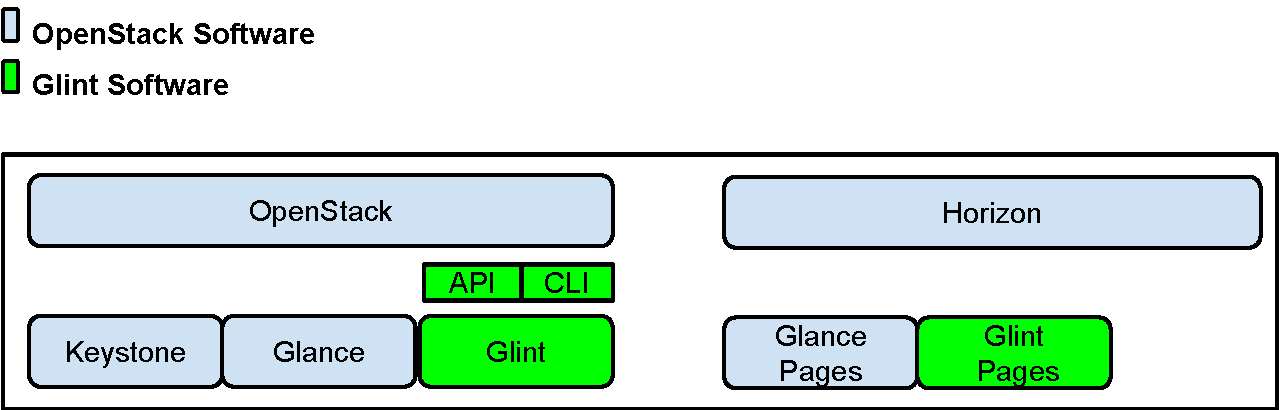
\includegraphics[width=36pc]{images/glintdesign.pdf}
\caption{\label{fig:glintfigure}Glint Software Components}
\end{center}
\end{figure}

There are 3 key functions the Glint service provides; Glint allows users to create remote sites representing a remote glance repository; Glint users can add their remote repository credentials for Glint management; Finally, Glint manages image distribution as specified by the user. Image management is the most complicated operation provided by Glint. Figure~\ref{fig:glintseqdiag} depicts the process of moving an image between two sites. 

\begin{figure}[H]
\begin{center}
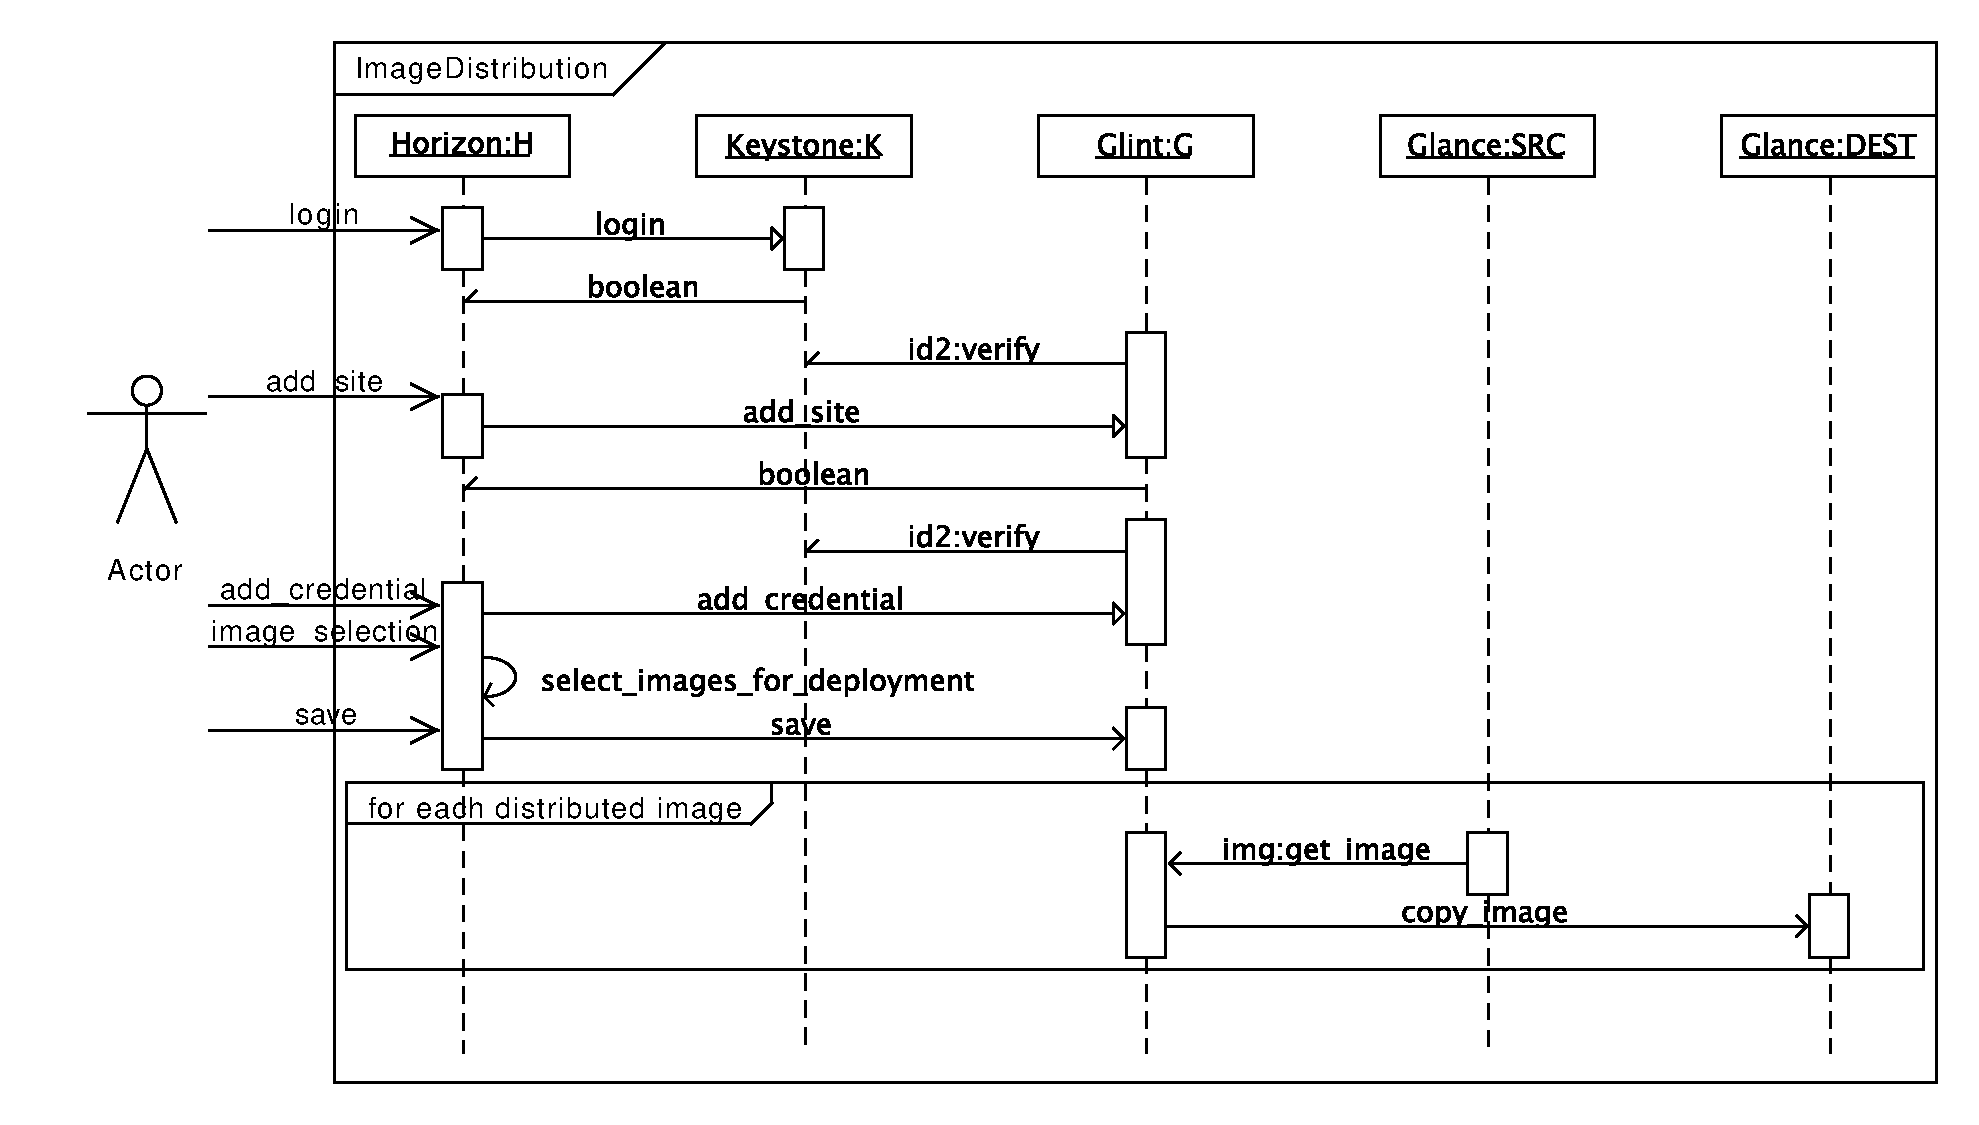
\includegraphics[width=36pc]{images/glintseqdiag.pdf}
\caption{\label{fig:glintseqdiag}Image Distribution Design}
\end{center}
\end{figure}

Glint is designed around OpenStack's Keystone service for user authenication. This design requires a user to have an OpenStack account on the site that Glint is using as its primary host. Therefore, the user must login and register with Glint which will then use Keystone to check if the user is valid (c.f., Figure~\ref{fig:glintlogin}). If the user is valid, Keystone will generate an authentication token that the glint service persists. User requests are then performed on behalf of glint using the token for authentication.

\begin{figure}[H]
\begin{center}
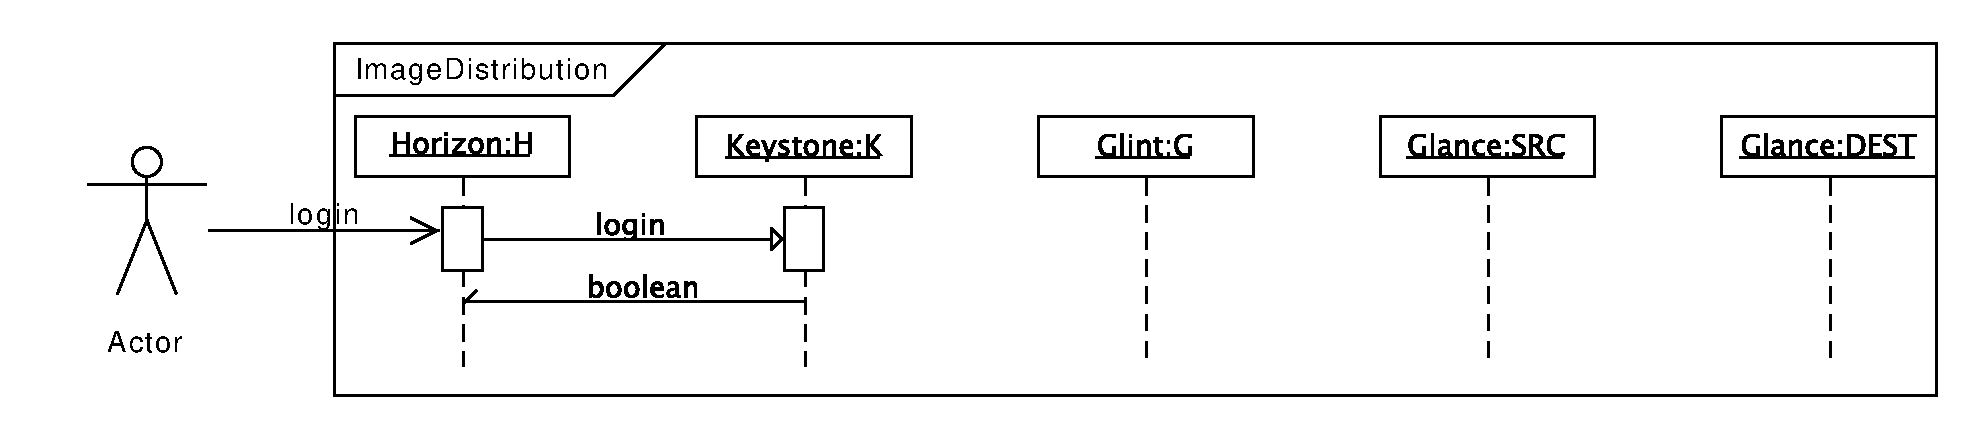
\includegraphics[width=36pc]{images/glintlogin.pdf}
\caption{\label{fig:glintlogin}Glint User Login}
\end{center}
\end{figure}

The concepts of remote OpenStack sites and remote site credentials is essential in the design of glint. Users can add remote sites as a source and destination of images. Site credentials can then be added so Glint can use the site without having to request input from the user every time the site is accessed. Figure~\ref{fig:glintsitecred} depicts the user adding a remote site to the glint service.

\begin{figure}[H]
\begin{center}
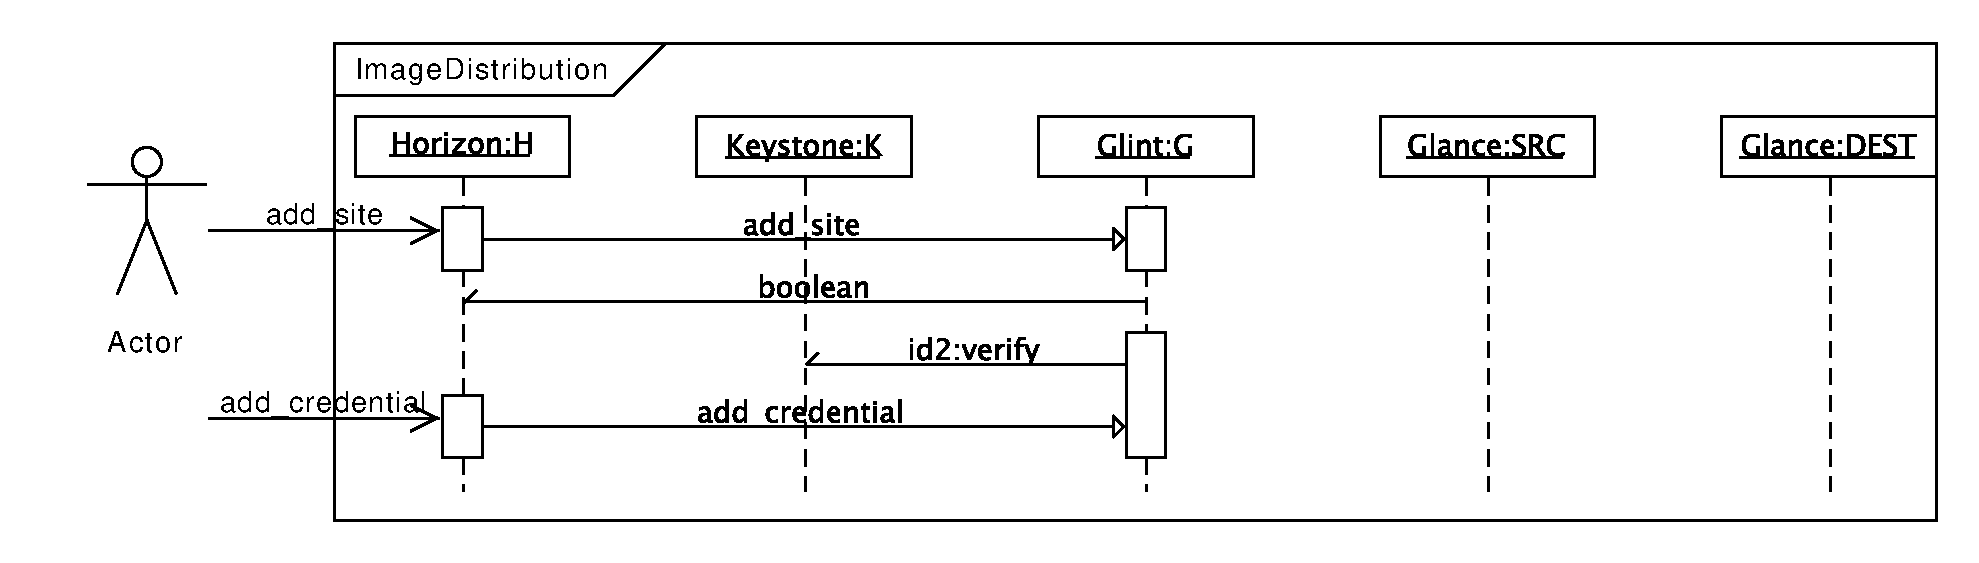
\includegraphics[width=36pc]{images/glintsitecred.pdf}
\caption{\label{fig:glintsitecred}Glint - Create remote site and add remote credential}
\end{center}
\end{figure}

OpenStack's Glance service provides the image copying and deleting functionality. Glint relies on this service to move images between remote sites. Figure~\ref{fig:glintdist} depicts the image distribution process. It requires the user to select which images they want on each site, once the user is happy they can save the new configuration. Glint proceeds to create a new thread for each image transfer or delete image operation. 

\begin{figure}[H]
\begin{center}
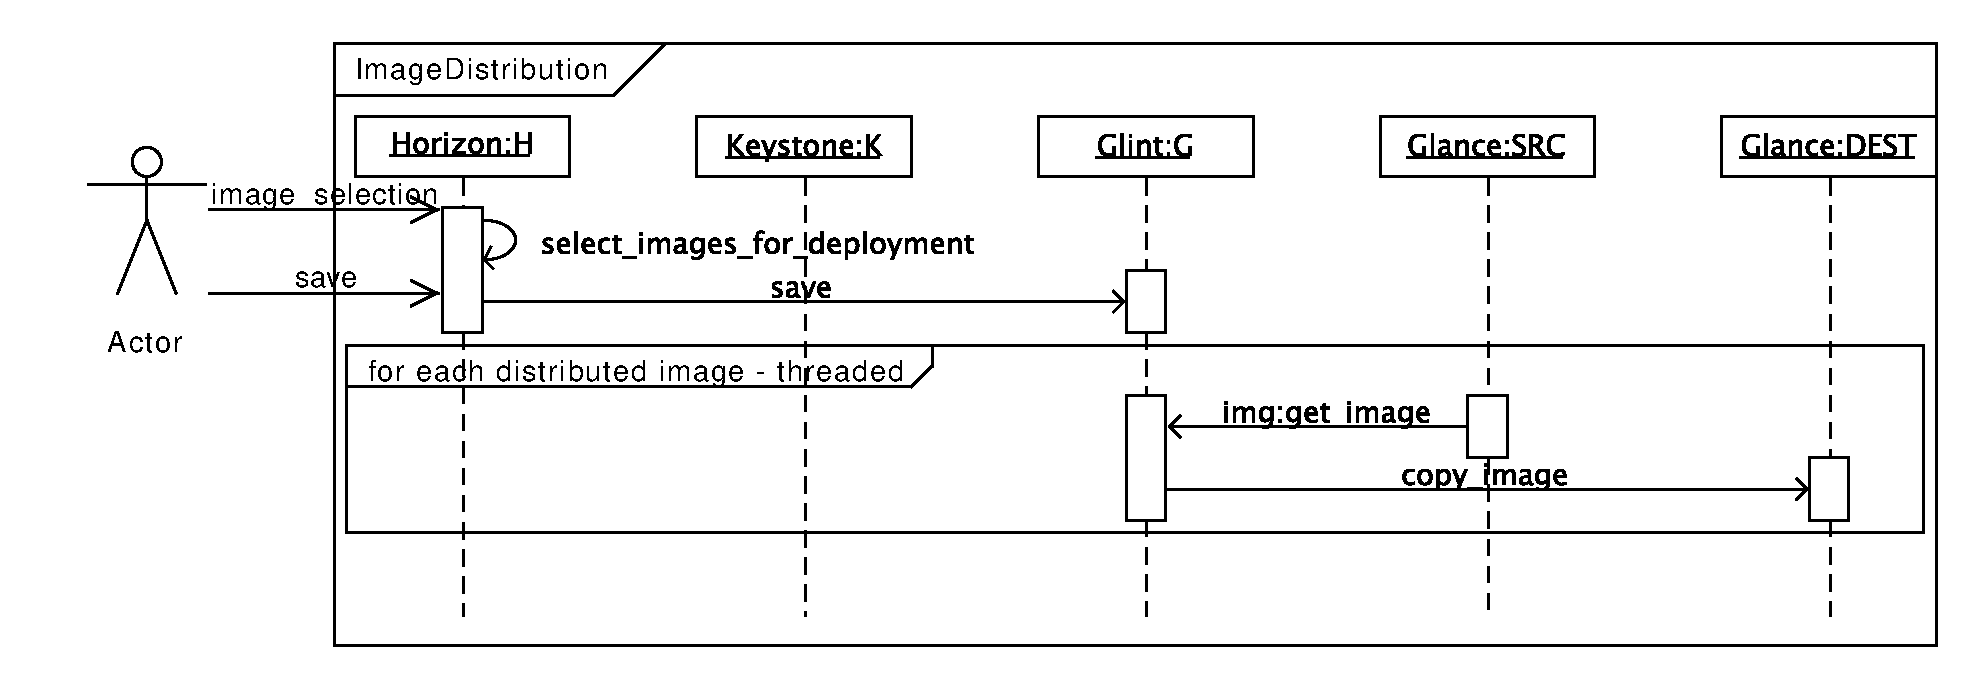
\includegraphics[width=36pc]{images/glintdist.pdf}
\caption{\label{fig:glintdist}Glint - Reconfigure Image Distribution}
\end{center}
\end{figure}

\section{Implementation}

Glint design and implementation follow the OpenStack framework. There are 4 main components developed and deployed to work with OpenStack. The image transfer component, the Application Programming Interface (API), the Command Line Interface (CLI) and the horizon web page elements. 

The image transfer component is an HTTP service that uses Openstack's Keystone and Glance services. The objective of the service is to integrate remote OpenStack clouds for the purpose of moving images seamlessly among them. The implementation is written in the python programming language and uses OpenStack's python APIs to integrate the Glance and Keystone services.

The API is written in python and provides users of the Glint service to construct their own applications using Glint. There are plans to provide Java and C/C++ APIs in the future.

The CLI is written in python and uses the API. The CLI is the first application to use the Glint API. The CLI provides all the functionality that is provided by the modified Horizon dashboard web pages added for Glint usage.

The modified Horizon dashboard is a set of added web pages to provide a friendly user interface within the familiar Horizon dashboard. The pages are added to the images management tab that Horizon already provides. 

The code for the 4 main components is managed within 2 Eclipse projects using the PyDev and Git plugins. The PyDev plugin understands the semantics of python and allows the Eclipse Graphical User Interface (GUI) to provide proper functionality that is relevant for python development. The Git plugin allows the use of Git and GitHub as our versioning system to track changes and maintain the projects. 

The first Eclipse project is a modified version of OpenStack's Horizon dashboard. This dashboard includes pages relevant to image distribution. Web pages in Horizon are described with python classes and use Django's powerful templating engine to provide a uniform presentation to the user. There are two extra pages added to provide image distribution. The first page allows users to add remote sites and add credentials to access remote sites. The second page allows users to view all images on all sites, and provides an interface to add or remove selected images from any site.

The second Eclipse project includes the API, CLI and the image transfer service. These are developed in python and can use either Django or Paste to serve HTTP requests. The Django-PyDev plugin is used for the project and provides Django related functions to manage the HTTP service component of the software. An API is provided for python to extend the functionality of the Glint service. The CLI is the first extension of the service that uses the API. The CLI is written in python and takes advantage of the ArgParse python module which makes it easier to develop CLI tools. The CLI and the modified Horizon interface are the two methods currently offered to interact with the image distribution service. The CLI and the Horizon interface are independent of each other, for example you can use the service with the CLI without having to install the modified Horizon dashboard.


\section{Deployment}

\subsection{Service Deployment}
It is recommended to deploy the Glint service to the same secure machine that the Keystone and Glance services are running. This is because glint maintains a database of user name, passwords and authentication tokens in it's database. So it is important to keep glint on a secure machine. Once glint is installed, you can use it immediately via the CLI.

Another deployment strategy is to also install the modified Horizon dashboard. This dashboard allows users of the local OpenStack site to add remote sites specific for themselves (i.e., other OpenStack sites the user has credentials on).  

\subsection{Image Deployment}
Figure~\ref{fig:glintfigure} depicts a basic deployment of an image using Glint with 3 OpenStack sites. Each OpenStack site is independent and has their own user and tenant management. The credentials of each site is stored on Glint securely and used by the service when the image deployment needs to be changed. For example, the user requested a deployment change such that Image A is to be duplicated from Site 1 to Site2 and Site3. Glint will first authenticate against Site1 using Keystone, then perform a copy operation for Site 2 and Site 3. For a successful copy operation, Glint will first authenticate the Site with credentials found in it's database for that site.

\begin{figure}[H]
\begin{center}
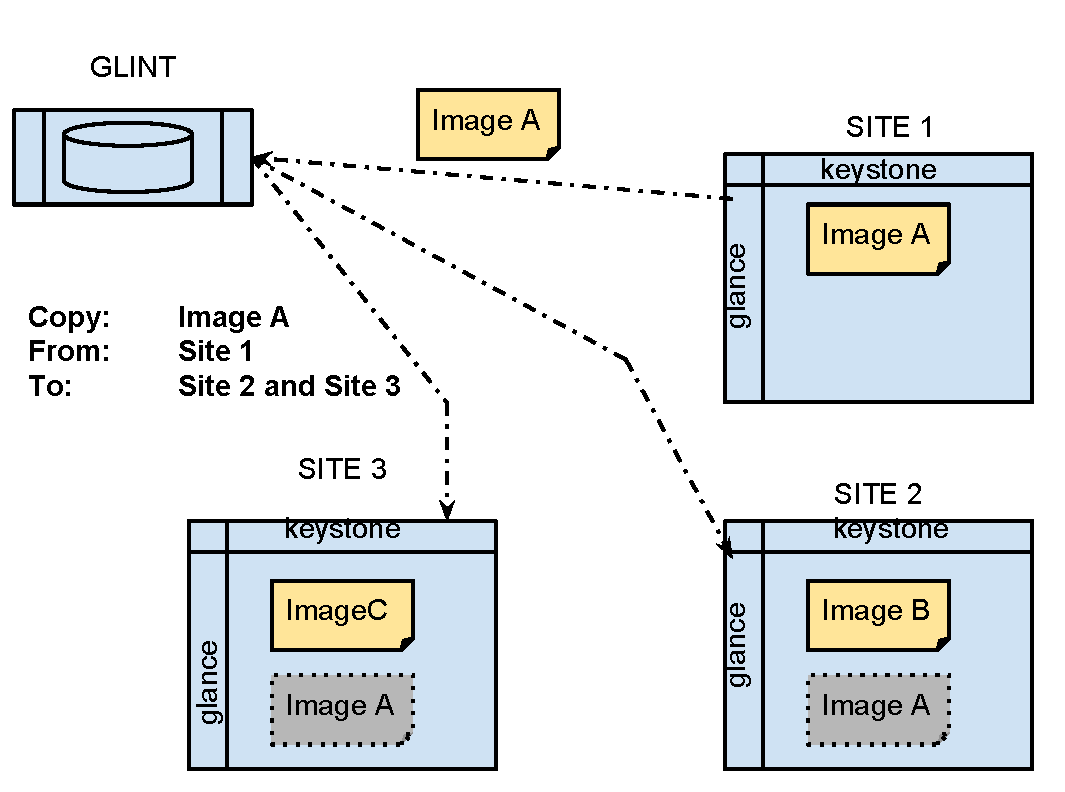
\includegraphics[width=36pc]{images/archglint.pdf}
\caption{\label{fig:glintfigure}Image Distribution }
\end{center}
\end{figure}



Glint is available on PyDev as required for deployment via StackForge for OpenStack integration. The latest version is currently deployed for image distribution at the University of Victoria. 

%%% \newpage

\section*{References}
\begin{thebibliography}{9}

\bibitem{vmdirac}  
VM dirac

\bibitem{chep:gable-talk}
Gable chep talk

\bibitem{chep:vac-vcycle}
VAC vcycle

\bibitem{hpcs:cloudpaper}
HPCS cloud paper

\bibitem{sobie-nyc-cloud}
Sobie NYC talk

\bibitem{ryan-chep}
Ryan CHEP talk

\bibitem{sobie-chep}
Sobie Belle-II talk


\bibitem{glint}
{\it Glint}, a system for managing VM images on multiple clouds.
https://github.com/hep-gc/glint

\end{thebibliography}

\end{document}